% ============================================================
%  ML IoT Lab – Presentation Template
%  HCMUT EE Machine Learning & IoT Lab
%  Faculty of Electrical & Electronics Engineering, HCMUT
%
%  Usage: compile with pdflatex (twice) or xelatex
% ============================================================

\documentclass[aspectratio=169, 10pt]{beamer}
\usepackage{newtxtext}
\usepackage{newtxmath}
\usepackage{beamerthemeMLIOT}   % custom theme (in same folder)
% thêm vô để gõ tiếng việt
\usepackage[utf8]{inputenc}
\usepackage[T5]{fontenc}


% ---- Additional packages ----
\usepackage{amsmath, amssymb}
\usepackage{booktabs}
\usepackage{multicol}
\usepackage{caption}
\usepackage{hyperref}
\usepackage[loadonly]{enumitem}
\usepackage{array}
\usepackage{pifont}
\usepackage{ragged2e}

% ---- Hyperlink colours ----
\hypersetup{
  colorlinks = true,
  urlcolor   = MLIOTaccent,
  linkcolor  = MLIOTblue,
  citecolor  = MLIOTblue
}

% ============================================================
%  Ký hiệu dùng lại nhiều lần trong bài
% ============================================================
% DeclareRobustCommand chứ KHÔNG phải newcommand.
% Hai lệnh này được dùng trong TIÊU ĐỀ BLOCK và ô bảng — đó là "đối số di động",
% nội dung bị mang đi dựng lại ở chỗ khác, ví dụ slide 11:
%     \begin{block}{Mười hai bài kiểm tra — 12/12 \xong}
% Lệnh mềm đặt vào đó có thể bung ra sai lúc dựng trang.
%
% Ghi cho rõ: đây KHÔNG phải nguyên nhân của lỗi "Runaway argument" ở slide 11.
% Lỗi đó là do \par nằm trong đối số của \textcolor — xem chú thích dưới đây.
% Đổi sang DeclareRobustCommand là phòng xa, không phải bản vá của lỗi ấy.
\DeclareRobustCommand{\xong}{\textcolor{MLIOTnavy}{\textbf{ĐẠT}}}
\DeclareRobustCommand{\chuaxong}{\textcolor{MLIOTcoral}{\textbf{chưa xong}}}

% Token đặc biệt: viết <pad> qua \textless/\textgreater cho chắc, vì dấu <, >
% đặt thẳng trong \texttt có thể ra ký tự khác tùy bảng mã font.
\DeclareRobustCommand{\tk}[1]{\texttt{\textless #1\textgreater}}

% Tên riêng nước ngoài có dấu KHÔNG thuộc bảng mã T5 (tiếng Việt) — ví dụ ć, ü.
% Đổi tạm sang T1 trong đúng phạm vi cái tên, nếu không pdflatex sẽ báo lỗi.
\newcommand{\tenlatin}[1]{{\fontencoding{T1}\selectfont #1}}

% Bảng trên slide luôn chật, thu hẹp khoảng cách cột lại cho vừa.
\newcommand{\bangchat}{\setlength{\tabcolsep}{3pt}}

% ============================================================
%  ĐỔI MÀU TRONG beamercolorbox: DÙNG {\color{X}...} CHỨ ĐỪNG \textcolor{X}{...}
% ============================================================
% \textcolor nhận đối số NGẮN — không cho phép ngắt đoạn. Đặt \par, dòng trắng,
% hay \begin{itemize} (itemize tự sinh \par) vào bên trong là vỡ ngay:
%
%     Runaway argument?
%     ! Paragraph ended before \@textcolor was complete.
%
% Và TeX báo lỗi ở dòng \end{frame} chứ không báo ở dòng gây ra, nên rất khó truy.
% Một khối hỏng đẻ ra cả chục lỗi dây chuyền — bản trước có 68 lỗi chỉ vì ba khối.
%
% \color là lệnh KHAI BÁO, đổi màu từ đó tới hết nhóm ngoặc, nên ngắt đoạn và
% itemize thoải mái. Số dấu ngoặc y hệt nên đổi qua lại không lệch:
%
%     \textcolor{MLIOTink}{...}   ->   {\color{MLIOTink}...}
%
% Cả 10 hộp trong file này đã đổi hết cho đồng nhất, không chỉ ba chỗ đang hỏng.

% ============================================================
%  PAPER METADATA – fill these in
% ============================================================
\title{Dịch máy Anh–Việt với Transformer tích hợp RoPE, RMSNorm và SwiGLU}

\author{%
  \textbf{\textcolor{MLIOTaccent}{Thái Nguyễn Thanh Phú}}%
  \texorpdfstring{\textcolor{MLIOTgold}{\textsuperscript{*a}}}{*a}\textcolor{MLIOTnavy}{,~}%
  \textbf{\textcolor{MLIOTnavy}{Trần Hải My}}%
  \texorpdfstring{\textcolor{MLIOTgold}{\textsuperscript{a}}}{a}\textcolor{MLIOTnavy}{,~}%
  \textbf{\textcolor{MLIOTnavy}{Mai Gia Bảo}}%
  \texorpdfstring{\textcolor{MLIOTgold}{\textsuperscript{a}}}{a}%
}


\setAffiliations{%
  \textsuperscript{*a}Ho Chi Minh University of Technology \\
  \textsuperscript{a}University of Information Technology%
}

\setCorrespondingAuthor{%
  *Corresponding/Presenting Author Email: \href{mailto:author@mail.com}{my.tran07@hcmut.edu.vn}%
}

\setPaperID{MLIOT-2026-XXX}

\institute{%
  Machine Learning \& IoT Lab,
  Ho Chi Minh City University of Technology (HCMUT)%
}

\date{June 2026}



% ============================================================
\begin{document}
% ============================================================

% ------------------------------------------------------------
%  SLIDE 1 – Title Slide
% ------------------------------------------------------------
\begin{frame}[plain]
  \titlepage
\end{frame}

% ------------------------------------------------------------
%  SLIDE 2 – Outline
% ------------------------------------------------------------
\begin{frame}{Outline}
	\begin{columns}[T]
		\begin{column}{0.55\textwidth}
			% This temporary font assignment scales the numbers perfectly
			\setbeamerfont{enumerate item}{size=\large}

			\begin{enumerate}
				\setlength{\itemsep}{0.7em} % Keeps a comfortable gap between items
				\item {\large Giới thiệu đề tài và mục tiêu}
				\item {\large Xử lý dữ liệu IWSLT 2015 En--Vi}
				\item {\large Kiến trúc Transformer tự viết}
				\item {\large Huấn luyện theo epoch \& đồng bộ Hugging Face}
				\item {\large Kết quả, chấm điểm và ablation}
				\item {\large Kết luận và tài liệu tham khảo}
			\end{enumerate}
		\end{column}
		\begin{column}{0.42\textwidth}
			\begin{block}{Contact Information}
				\footnotesize
				\textbf{\textcolor{MLIOTnavy}{Address:}}~403.1 BK.B6, HCMUT Campus 2\\[0.35em]
				\textbf{\textcolor{MLIOTnavy}{Email:}}\\
				nkloi@hcmut.edu.vn\\
				mlandiotlab@gmail.com\\[0.35em]
				\textbf{\textcolor{MLIOTnavy}{Website:}}~mliotlab.com\\[0.35em]
				\textbf{\textcolor{MLIOTnavy}{Facebook:}}~facebook.com/hcmut.ml.iot.lab\\[0.35em]
				\textbf{\textcolor{MLIOTnavy}{YouTube:}}~youtube.com/@mliotlab
			\end{block}
		\end{column}
	\end{columns}
\end{frame}

% ------------------------------------------------------------
%  SLIDE 3 – Giới thiệu đề tài
% ------------------------------------------------------------
\begin{frame}[shrink=10]{Giới thiệu đề tài}
  \begin{columns}[T]
    \begin{column}{0.51\textwidth}
      \begin{block}{Bài toán}
        Xây dựng hệ thống dịch máy nơ-ron \textbf{Anh $\rightarrow$ Việt} hoàn chỉnh,
        từ tầng toán học tới tầng dịch vụ chạy được.
        \begin{itemize}
          \setlength{\itemsep}{0.2em}
          \item Dữ liệu IWSLT 2015 En--Vi (phụ đề TED): \textbf{131.339} cặp câu sau làm sạch.
          \item Ngữ liệu ít hơn WMT hàng trăm lần $\rightarrow$ \textbf{chống quá khớp}
            là bài toán trung tâm.
          \item Tiếng Việt nhiều dấu thanh $\rightarrow$ chuẩn hóa Unicode NFC là bắt buộc.
        \end{itemize}
      \end{block}
      \begin{block}{Hạ tầng thực tế}
        \begin{itemize}
          \setlength{\itemsep}{0.2em}
          \item GPU Kaggle \textbf{Tesla T4} bản miễn phí, phiên bị ngắt bất kỳ lúc nào.
          \item Vì vậy \textbf{checkpoint chịu lỗi} là yêu cầu bắt buộc, không phải
            tính năng thêm.
        \end{itemize}
      \end{block}
    \end{column}
    \begin{column}{0.46\textwidth}
      \begin{block}{Ràng buộc nhóm tự đặt ra}
        Toàn bộ kiến trúc \textbf{do nhóm tự cài bằng PyTorch thuần}.
        Trong \texttt{src/} tuyệt đối \textbf{không} dùng:
        \begin{itemize}
          \setlength{\itemsep}{0.15em}
          \item \texttt{nn.Transformer}, \texttt{nn.MultiheadAttention}
          \item \texttt{F.scaled\_dot\_product\_attention}
          \item \texttt{nn.LayerNorm} / \texttt{nn.RMSNorm}
          \item mô hình pretrained, và không gọi API mô hình ngôn ngữ lớn
        \end{itemize}
        Lớp tham chiếu của PyTorch \textbf{chỉ} xuất hiện trong \texttt{tests/} để
        đối chiếu số học.
      \end{block}
      \begin{beamercolorbox}[wd=\textwidth, rounded=true, sep=6pt]{block body alerted}
        {\color{MLIOTink}\footnotesize\textbf{Nguyên tắc xuyên suốt:} mọi lựa chọn
        kiến trúc phải chứng minh được bằng \textbf{số liệu thực nghiệm}, không lấy
        mặc định của bài báo làm kết luận.}
      \end{beamercolorbox}
    \end{column}
  \end{columns}
\end{frame}

% ------------------------------------------------------------
%  SLIDE 4 – Mục tiêu
% ------------------------------------------------------------
\begin{frame}[shrink=10]{Mục tiêu}
  \begin{columns}[T]
    \begin{column}{0.48\textwidth}
      \begin{block}{Mục tiêu kỹ thuật}
        Xây dựng Transformer hiện đại dịch Anh $\rightarrow$ Việt \textbf{từ con số 0}:
        \begin{itemize}
          \setlength{\itemsep}{0.15em}
          \item \textbf{RoPE} — mã hóa vị trí xoay
          \item \textbf{Pre-Norm} — chuẩn hóa trước khối con
          \item \textbf{RMSNorm} — chuẩn hóa theo căn trung bình bình phương
          \item \textbf{SwiGLU} — feed-forward có cổng
          \item Bộ kiểm tra tính đúng đắn của kiến trúc
          \item Checkpoint chịu lỗi qua Hugging Face Hub
          \item Chấm điểm BLEU và chrF++ bằng sacrebleu
          \item Triển khai Docker và đo độ trễ
        \end{itemize}
      \end{block}
    \end{column}
    \begin{column}{0.49\textwidth}
      \begin{block}{Tiêu chí đo được (\textit{Xong khi})}
        \scriptsize\bangchat
        \begin{tabular}{@{}p{4.0cm}p{2.1cm}@{}}
          \toprule
          \textbf{Hạng mục} & \textbf{Ngưỡng} \\
          \midrule
          Kiểm tra đúng đắn kiến trúc  & 12/12 bài đạt \\
          Đối chiếu tham chiếu PyTorch & lệch $< 10^{-5}$ \\
          Học thuộc 50 câu (cổng chặn) & loss $< 0{,}05$ \\
          Huấn luyện liên tục          & không có NaN \\
          Giết phiên rồi phục hồi      & lệch $< 1\%$ \\
          Thời gian đồng bộ checkpoint & $< 5\%$ tổng \\
          BLEU trên tst2013            & $\ge 19$ \\
          \bottomrule
        \end{tabular}
      \end{block}
      \begin{beamercolorbox}[wd=\textwidth, rounded=true, sep=6pt]{block body alerted}
        {\color{MLIOTink}\footnotesize Mức đánh giá BLEU trên tst2013:
        $\ge 19$ tối thiểu chấp nhận · $\ge 22$ tốt · $\ge 29$ rất tốt.}
      \end{beamercolorbox}
    \end{column}
  \end{columns}
\end{frame}

% ------------------------------------------------------------
%  SLIDE 5 – Tổng quan pipeline
% ------------------------------------------------------------
\begin{frame}[shrink=10]{Tổng quan pipeline}
  \begin{methodcols}
    \methodcol{\ding{202}~Dữ liệu}{%
      \begin{itemize}
        \setlength{\itemsep}{0.1em}
        \item Tải IWSLT 2015 En--Vi
        \item Chuẩn hóa NFC, lọc 5 bước
        \item Kiểm tra rò rỉ test vào train
        \item BPE 32k dùng chung En + Vi
        \item Gom batch theo độ dài
      \end{itemize}%
    }
    \methodcol{\ding{203}~Mô hình}{%
      \begin{itemize}
        \setlength{\itemsep}{0.1em}
        \item Encoder--Decoder 6 + 6 lớp
        \item Attention tự viết + RoPE
        \item RMSNorm, Pre-Norm
        \item Feed-forward SwiGLU
        \item Chia sẻ embedding ba nơi
      \end{itemize}%
    }
    \methodcol{\ding{204}~Huấn luyện \& Đánh giá}{%
      \begin{itemize}
        \setlength{\itemsep}{0.1em}
        \item AdamW, fp16 + GradScaler
        \item Cộng dồn gradient 4 bước
        \item Đánh giá dev mỗi 1000 bước
        \item Checkpoint lên HF Hub
        \item BLEU, chrF++ (sacrebleu)
      \end{itemize}%
    }
  \end{methodcols}

  \vspace{0.5em}
  \begin{center}
    \begin{beamercolorbox}[wd=0.93\textwidth, rounded=true, sep=5pt,
          center]{block body}
      \footnotesize
      \texttt{prepare\_data} $\rightarrow$ \texttt{train\_tokenizer} $\rightarrow$
      \texttt{overfit\_sanity} \textit{(cổng chặn)} $\rightarrow$
      \texttt{benchmark\_speed} $\rightarrow$ \texttt{train} $\rightarrow$
      \texttt{evaluate}
    \end{beamercolorbox}
  \end{center}
\end{frame}

% ------------------------------------------------------------
%  SLIDE 6 – Xử lý dữ liệu (1/2)
% ------------------------------------------------------------
\begin{frame}[shrink=10]{Xử lý dữ liệu (1/2) — Làm sạch và chống rò rỉ}
  \begin{columns}[T]
    \begin{column}{0.46\textwidth}
      \begin{block}{Năm bước lọc, giữ đúng thứ tự}
        \begin{enumerate}
          \setlength{\itemsep}{0.1em}
          \item Chuẩn hóa Unicode về \textbf{NFC} — bắt buộc với tiếng Việt
          \item Bỏ dòng rỗng
          \item Bỏ cặp câu trùng lặp
          \item Bỏ câu dài quá \textbf{100} token
          \item Bỏ cặp lệch độ dài quá \textbf{3} lần
        \end{enumerate}
        \vspace{0.2em}
        Tập dev/test \textbf{không bị lọc}, chỉ chuẩn hóa NFC để giữ nguyên số câu.
      \end{block}
      \begin{beamercolorbox}[wd=\textwidth, rounded=true, sep=6pt]{block body alerted}
        {\color{MLIOTink}\footnotesize\textbf{Chống rò rỉ:} 12 cặp câu của tst2012
        và 12 cặp của tst2013 trùng nguyên si trong train $\rightarrow$ xóa
        \textbf{24 cặp} khỏi \textit{train}, không đụng dev/test. Bỏ qua bước này là
        điểm BLEU bị đội lên giả tạo.}
      \end{beamercolorbox}
    \end{column}
    \begin{column}{0.5\textwidth}
      \begin{block}{Bảng thống kê lọc}
        \scriptsize\bangchat
        \begin{tabular}{@{}lrrrr@{}}
          \toprule
          \textbf{Split} & \textbf{Trước} & \textbf{Sau} & \textbf{Bị loại} &
          \textbf{Tỉ lệ} \\
          \midrule
          train   & 133.317 & 131.339 & 1.978 & 1{,}48\% \\
          tst2012 & 1.553   & 1.553   & 0     & 0\% \\
          tst2013 & 1.268   & 1.268   & 0     & 0\% \\
          \bottomrule
        \end{tabular}
        \par\vspace{0.4em}
        Chi tiết 1.978 cặp bị loại khỏi train: 151 rỗng · 1.006 trùng ·
        760 quá dài · 40 lệch độ dài · 21 rò rỉ.
      \end{block}
      \begin{block}{Token đặc biệt — ID cố định}
        \footnotesize
        \tk{pad} $=0$ \quad \tk{unk} $=1$ \quad \tk{bos} $=2$ \quad \tk{eos} $=3$
        \par\vspace{0.3em}
        Chốt dùng \tk{bos}/\tk{eos}, dành sẵn \tk{2en} và \tk{2vi} cho hướng gộp hai
        chiều dịch sau này.
      \end{block}
    \end{column}
  \end{columns}
\end{frame}

% ------------------------------------------------------------
%  SLIDE 7 – Xử lý dữ liệu (2/2)
% ------------------------------------------------------------
\begin{frame}[shrink=10]{Xử lý dữ liệu (2/2) — Tokenizer và đóng gói batch}
  \begin{columns}[T]
    \begin{column}{0.47\textwidth}
      \begin{block}{BPE 32k dùng chung En + Vi}
        \begin{itemize}
          \setlength{\itemsep}{0.15em}
          \item Một bộ từ vựng \textbf{32.000} token cho cả hai ngôn ngữ
          \item Nhờ vậy encoder, decoder và lớp xuất \textbf{chia sẻ chung một ma trận
            embedding}, tiết kiệm \textbf{16{,}4 triệu} tham số
        \end{itemize}
      \end{block}
      \begin{block}{Chất lượng tokenizer}
        \scriptsize\bangchat
        \begin{tabular}{@{}lr@{}}
          \toprule
          \textbf{Chỉ số} & \textbf{Giá trị} \\
          \midrule
          Fertility tiếng Anh          & 1{,}0664 token/từ \\
          Fertility tiếng Việt         & 1{,}0137 token/từ \\
          Tỉ lệ \tk{unk} trên train    & 0{,}0000\% \\
          Tỉ lệ \tk{unk} trên dev      & 0{,}0000\% \\
          \bottomrule
        \end{tabular}
        \par\vspace{0.3em}
        Fertility gần 1 nghĩa là hầu hết từ vẫn là \textbf{một} token, không bị băm vụn.
      \end{block}
    \end{column}
    \begin{column}{0.49\textwidth}
      \begin{block}{Đóng gói batch theo số token}
        \begin{itemize}
          \setlength{\itemsep}{0.15em}
          \item Batch tính theo \textbf{4096 token}, không theo số câu
            $\rightarrow$ tải GPU đều giữa các bước
          \item \textbf{Gom theo độ dài}: câu dài xấp xỉ nhau vào cùng batch
            $\rightarrow$ giảm mạnh ô \tk{pad} lãng phí
          \item Sinh sẵn \textbf{padding mask} và \textbf{causal mask}
        \end{itemize}
      \end{block}
      \begin{block}{Tái lập được — không phải chuyện nhỏ}
        \begin{itemize}
          \setlength{\itemsep}{0.15em}
          \item Cố định seed cho \texttt{torch}, \texttt{numpy}, \texttt{random} và cả
            worker của DataLoader
          \item Thứ tự batch mỗi epoch ghim theo cặp \textbf{(seed, epoch)}
          \item Khi phiên bị ngắt giữa epoch, lượt sau tua nhanh qua đúng số batch đã
            tiêu thụ và gặp lại \textbf{đúng thứ tự batch cũ}
        \end{itemize}
      \end{block}
    \end{column}
  \end{columns}
\end{frame}

% ------------------------------------------------------------
%  SLIDE 8 – Kiến trúc (1/3)
% ------------------------------------------------------------
\begin{frame}[shrink=10]{Kiến trúc (1/3) — Tổng quan mô hình}
  \begin{columns}[T]
    \begin{column}{0.49\textwidth}
      \begin{block}{Luồng dữ liệu}
        \scriptsize\bangchat
        \begin{tabular}{@{}ll@{}}
          \toprule
          \multicolumn{2}{@{}l}{\textbf{ENCODER} \quad vào: \texttt{src\_ids}
            $(B, S)$} \\
          \midrule
          Embedding chung   & $(B, S, 512)$ \\
          $6 \times$ lớp    & self-attention — \textbf{có RoPE} \\
                            & feed-forward SwiGLU \\
          \textit{ra}       & bộ nhớ $(B, S, 512)$ \\
          \midrule
          \multicolumn{2}{@{}l}{\textbf{DECODER} \quad vào: \texttt{tgt\_ids}
            $(B, T)$} \\
          \midrule
          Embedding chung   & $(B, T, 512)$ \\
          $6 \times$ lớp    & self-attention — \textbf{có RoPE} \\
                            & cross-attention — \textbf{KHÔNG RoPE} \\
                            & feed-forward SwiGLU \\
          RMSNorm cuối      & \\
          Linear chia sẻ    & $(B, T, 32000)$ \\
          \bottomrule
        \end{tabular}
      \end{block}
    \end{column}
    \begin{column}{0.48\textwidth}
      \begin{block}{Bảng đếm tham số}
        \scriptsize\bangchat
        \begin{tabular}{@{}lr@{}}
          \toprule
          \textbf{Thành phần} & \textbf{Số tham số} \\
          \midrule
          Embedding (dùng chung) & 16.384.000 \\
          Encoder (6 lớp)        & 12.638.720 \\
          Decoder (6 lớp)        & 18.933.248 \\
          Lớp xuất               & 0 \textit{(chia sẻ)} \\
          \midrule
          \textbf{Tổng}          & \textbf{47.955.968} \\
          \bottomrule
        \end{tabular}
      \end{block}
      \begin{block}{Siêu tham số đã chốt}
        \scriptsize\bangchat
        \begin{tabular}{@{}ll@{}}
          \toprule
          \texttt{d\_model} & 512 \\
          Số head           & 8 (mỗi head 64 chiều) \\
          Số lớp            & 6 encoder + 6 decoder \\
          \texttt{d\_ff}    & 688 (SwiGLU) \\
          Dropout           & 0{,}3 — cao vì dữ liệu ít \\
          Từ vựng           & 32.000 chung En + Vi \\
          Khởi tạo          & Xavier \\
          \bottomrule
        \end{tabular}
      \end{block}
    \end{column}
  \end{columns}
\end{frame}

% ------------------------------------------------------------
%  SLIDE 9 – Kiến trúc (2/3)
% ------------------------------------------------------------
\begin{frame}[shrink=10]{Kiến trúc (2/3) — Bốn khối hiện đại, mỗi khối hai phương án}
  \begin{columns}[T]
    \begin{column}{0.51\textwidth}
      \begin{block}{Công thức đã cài}
        \footnotesize
        % Bóp sát khoảng trắng quanh công thức, slide chật chỗ.
        \setlength{\abovedisplayskip}{3pt}\setlength{\belowdisplayskip}{3pt}
        \setlength{\abovedisplayshortskip}{3pt}\setlength{\belowdisplayshortskip}{3pt}
        \textbf{RMSNorm} — bỏ hẳn phép trừ trung bình của LayerNorm:
        \[
          \mathrm{RMSNorm}(x) =
          \frac{x}{\sqrt{\frac{1}{d}\sum_{i=1}^{d} x_i^{2} + \epsilon}} \odot g
        \]
        \textbf{SwiGLU} — feed-forward có cổng, dùng ba ma trận:
        \[
          \mathrm{SwiGLU}(x) = \big(\mathrm{Swish}(xW_1) \odot xW_3\big) W_2
        \]
        \textbf{Pre-Norm} — chuẩn hóa \textit{trước} khối con, đường residual
        thông suốt: $x_{\ell+1} = x_{\ell} + \mathrm{SubLayer}(\mathrm{Norm}(x_{\ell}))$.
        \par\vspace{0.3em}
        \textbf{RoPE} — xoay từng cặp chiều của $q$ và $k$ theo vị trí, nên tích vô
        hướng chỉ còn phụ thuộc \textbf{khoảng cách tương đối} $m - n$.
      \end{block}
    \end{column}
    \begin{column}{0.46\textwidth}
      \begin{block}{Đổi kiến trúc bằng một dòng YAML}
        \footnotesize
        \begin{itemize}
          \setlength{\itemsep}{0.1em}
          \item \textbf{A1} Chuẩn hóa: \texttt{rmsnorm} / \texttt{layernorm}
          \item \textbf{A4} Mã hóa vị trí: \texttt{rope} / \texttt{sinusoidal}
          \item \textbf{A5} Feed-forward: \texttt{swiglu} / \texttt{relu}
          \item \textbf{A6} Vị trí chuẩn hóa: \texttt{pre} / \texttt{post}
          \item \textbf{A2} Warmup: tắt / bật
          \item \textbf{A3} Label smoothing: $0{,}0$ / $0{,}1$
        \end{itemize}
        \vspace{0.2em}
        Đổi giá trị trong YAML là đổi kiến trúc — \textbf{không sửa dòng code nào}.
        Nhờ vậy mỗi thí nghiệm ablation chỉ khác \textbf{đúng một yếu tố}.
      \end{block}
      \begin{beamercolorbox}[wd=\textwidth, rounded=true, sep=6pt]{block body alerted}
        {\color{MLIOTink}\footnotesize Warmup và Label Smoothing \textbf{mặc định
        TẮT}. Giữ hay bỏ do \textbf{kết quả ablation} quyết định, không phải do bài
        báo quyết định.}
      \end{beamercolorbox}
    \end{column}
  \end{columns}
\end{frame}


% ------------------------------------------------------------
%  SLIDE 11 – Kiểm chứng tính đúng đắn
% ------------------------------------------------------------
\begin{frame}[shrink=10]{Kiểm chứng tính đúng đắn kiến trúc}
  \begin{columns}[T]
    \begin{column}{0.5\textwidth}
      \begin{block}{Mười hai bài kiểm tra — 12/12 \xong}
        \scriptsize\bangchat
        \begin{tabular}{@{}rp{5.4cm}@{}}
          \toprule
          \textbf{\#} & \textbf{Kiểm điều gì} \\
          \midrule
          1  & Causal mask không cho nhìn về sau \\
          2  & Padding mask có tác dụng \\
          3  & Trọng số attention hợp lệ \\
          4  & RoPE mã hóa đúng vị trí tương đối \\
          5  & Gradient chảy tới mọi tham số, không NaN \\
          6  & Đối chiếu số với tham chiếu PyTorch \\
          7  & \textbf{Học thuộc 50 câu} (cổng chặn Phase 2) \\
          8  & RMSNorm chuẩn hóa đúng công thức \\
          9  & SwiGLU đúng công thức, đúng số tham số \\
          10 & Residual Pre-Norm thông suốt, có norm cuối \\
          11 & RoPE không bị áp vào cross-attention \\
          12 & Mô hình chạy đúng ở fp16 \\
          \bottomrule
        \end{tabular}
        \par\vspace{0.3em}
        Bài 6 đối chiếu RMSNorm tự viết với \texttt{torch.nn.RMSNorm} và lõi attention
        với \texttt{F.scaled\_dot\_product\_attention}, yêu cầu lệch $< 10^{-5}$.
      \end{block}
    \end{column}
    \begin{column}{0.47\textwidth}
      \begin{center}
        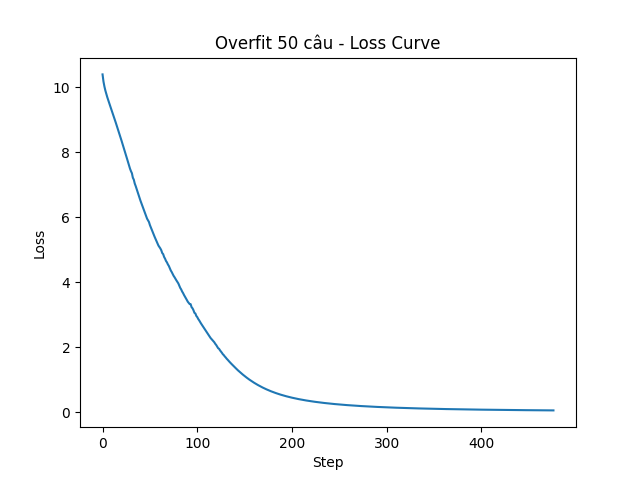
\includegraphics[width=0.78\textwidth]{overfit_loss.png}
      \end{center}
      \vspace{-0.4em}
      {\scriptsize\textit{Hình 1: Cổng chặn "học thuộc 50 câu" — loss về gần 0 trong
      chưa tới 500 bước.}}
      \vspace{0.4em}
      \begin{beamercolorbox}[wd=\textwidth, rounded=true, sep=6pt]{block body alerted}
        {\color{MLIOTink}\scriptsize\textbf{Cổng chặn:} loss cuối $< 0{,}05$
        \xong{}, BLEU trên chính 50 câu đó \textbf{100{,}00} \xong{}. Không học
        thuộc nổi 50 câu là kiến trúc còn sai — chưa qua thì chưa được huấn luyện.}
      \end{beamercolorbox}
    \end{column}
  \end{columns}
\end{frame}


% ------------------------------------------------------------
%  SLIDE 13 – Huấn luyện theo epoch
% ------------------------------------------------------------
\begin{frame}[shrink=15]{Huấn luyện theo epoch — một chu kỳ cập nhật}
  \begin{columns}[T]
    \begin{column}{0.48\textwidth}
      \begin{block}{Cấu hình tối ưu}
        \scriptsize\bangchat
        \begin{tabular}{@{}ll@{}}
          \toprule
          Optimizer         & AdamW, $\beta = (0{,}9\,;\,0{,}98)$, wd $0{,}01$ \\
          Learning rate     & $7 \times 10^{-4}$, lịch \textbf{cố định} \\
          Label smoothing   & $0{,}0$ \\
          Cộng dồn gradient & 4 micro-batch \\
          Cắt gradient      & theo norm $1{,}0$ \\
          Độ chính xác      & fp16 + GradScaler \\
          \bottomrule
        \end{tabular}
      \end{block}
    \end{column}
    \begin{column}{0.48\textwidth}
      \begin{block}{Nhịp của một epoch}
        \begin{itemize}
          \setlength{\itemsep}{0.15em}
          \item Một epoch $=$ \textbf{177} bước optimizer
          \item Mỗi \textbf{50} bước: ghi log loss, learning rate, giây/bước,
            token/giây
          \item Mỗi \textbf{1.000} bước: đánh giá trên dev (tst2012), tính loss dev và
            perplexity
          \item Tốt hơn kỷ lục $\rightarrow$ lưu \texttt{tot\_nhat.pt} và đẩy lên Hub
            ngay
          \item Mỗi \textbf{2.000} bước: lưu \texttt{moi\_nhat.pt} để chạy tiếp
          \item \textbf{Dừng sớm} sau 5 lần đánh giá liên tiếp không cải thiện
        \end{itemize}
      \end{block}
      \begin{block}{Ngân sách thời gian mỗi phiên}
        \begin{itemize}
          \setlength{\itemsep}{0.15em}
          \item Trainer nhận thêm \textbf{giới hạn giờ} cho mỗi phiên Kaggle
          \item Hết giờ $\rightarrow$ tự lưu, đẩy lên Hub rồi dừng \textbf{sạch sẽ}
          \item Phiên sau chỉ cần cờ \texttt{-{}-tiep-tuc} là chạy tiếp đúng chỗ cũ,
            kể cả trên \textbf{máy của người khác}
        \end{itemize}
      \end{block}
    \end{column}
  \end{columns}
\end{frame}

% ------------------------------------------------------------
%  SLIDE 14 – Checkpoint & Hugging Face
% ------------------------------------------------------------
\begin{frame}[shrink=15]{Checkpoint chịu lỗi và đồng bộ Hugging Face Hub}
  \begin{columns}[T]
    \begin{column}{0.48\textwidth}
      \begin{block}{Bảy món phải lưu — thiếu một là resume sai mà không báo lỗi}
        \scriptsize\bangchat
        \begin{tabular}{@{}p{2.6cm}p{3.6cm}@{}}
          \toprule
          \textbf{Món} & \textbf{Thiếu thì hỏng thế nào} \\
          \midrule
          Trọng số mô hình      & mất toàn bộ tiến trình học \\
          Trạng thái optimizer  & momentum về 0, loss giật lên \\
          Trạng thái scheduler  & learning rate nhảy về đầu \\
          Trạng thái GradScaler & hệ số giãn fp16 sai nhịp \\
          Số bước, số epoch     & không biết đang ở đâu \\
          Bản sao cấu hình      & không dựng lại đúng mô hình \\
          Seed + trạng thái RNG & dropout, thứ tự batch khác đi \\
          \bottomrule
        \end{tabular}
      \end{block}
      \begin{block}{Ghi file an toàn}
        \footnotesize
        Ghi ra file tạm rồi mới \textbf{đổi tên}. Ghi đè trực tiếp mà phiên Kaggle chết
        đúng lúc đang ghi thì mất luôn \textbf{cả bản cũ lẫn bản mới}.
      \end{block}
    \end{column}
    \begin{column}{0.48\textwidth}
      \begin{block}{Bố cục repo trên Hugging Face Hub}
        \scriptsize
        \texttt{checkpoints/}\tk{ten\_chay}\texttt{/moi\_nhat.pt} — bản mới nhất, để
        chạy tiếp \\
        \texttt{checkpoints/}\tk{ten\_chay}\texttt{/tot\_nhat.pt} — bản tốt nhất theo
        loss dev \\
        \texttt{logs/}\tk{ten\_chay}\texttt{/metrics.csv} — đường loss liền mạch qua
        các phiên \\
        \texttt{configs/}\tk{ten\_chay}\texttt{.yaml} — cấu hình đã gộp \\
        \texttt{artifacts/tokenizer/tokenizer.json} — dùng chung mọi lượt \\
        \texttt{smoke/...} — smoke test, \textbf{không} phải kết quả thật
      \end{block}
    \end{column}
  \end{columns}
\end{frame}

% ------------------------------------------------------------
%  SLIDE 15 – Thí nghiệm giết phiên và phục hồi
% ------------------------------------------------------------
\begin{frame}[shrink=10]{Thí nghiệm giết phiên và phục hồi}
  \begin{columns}[T]
    \begin{column}{0.55\textwidth}
      \begin{center}
        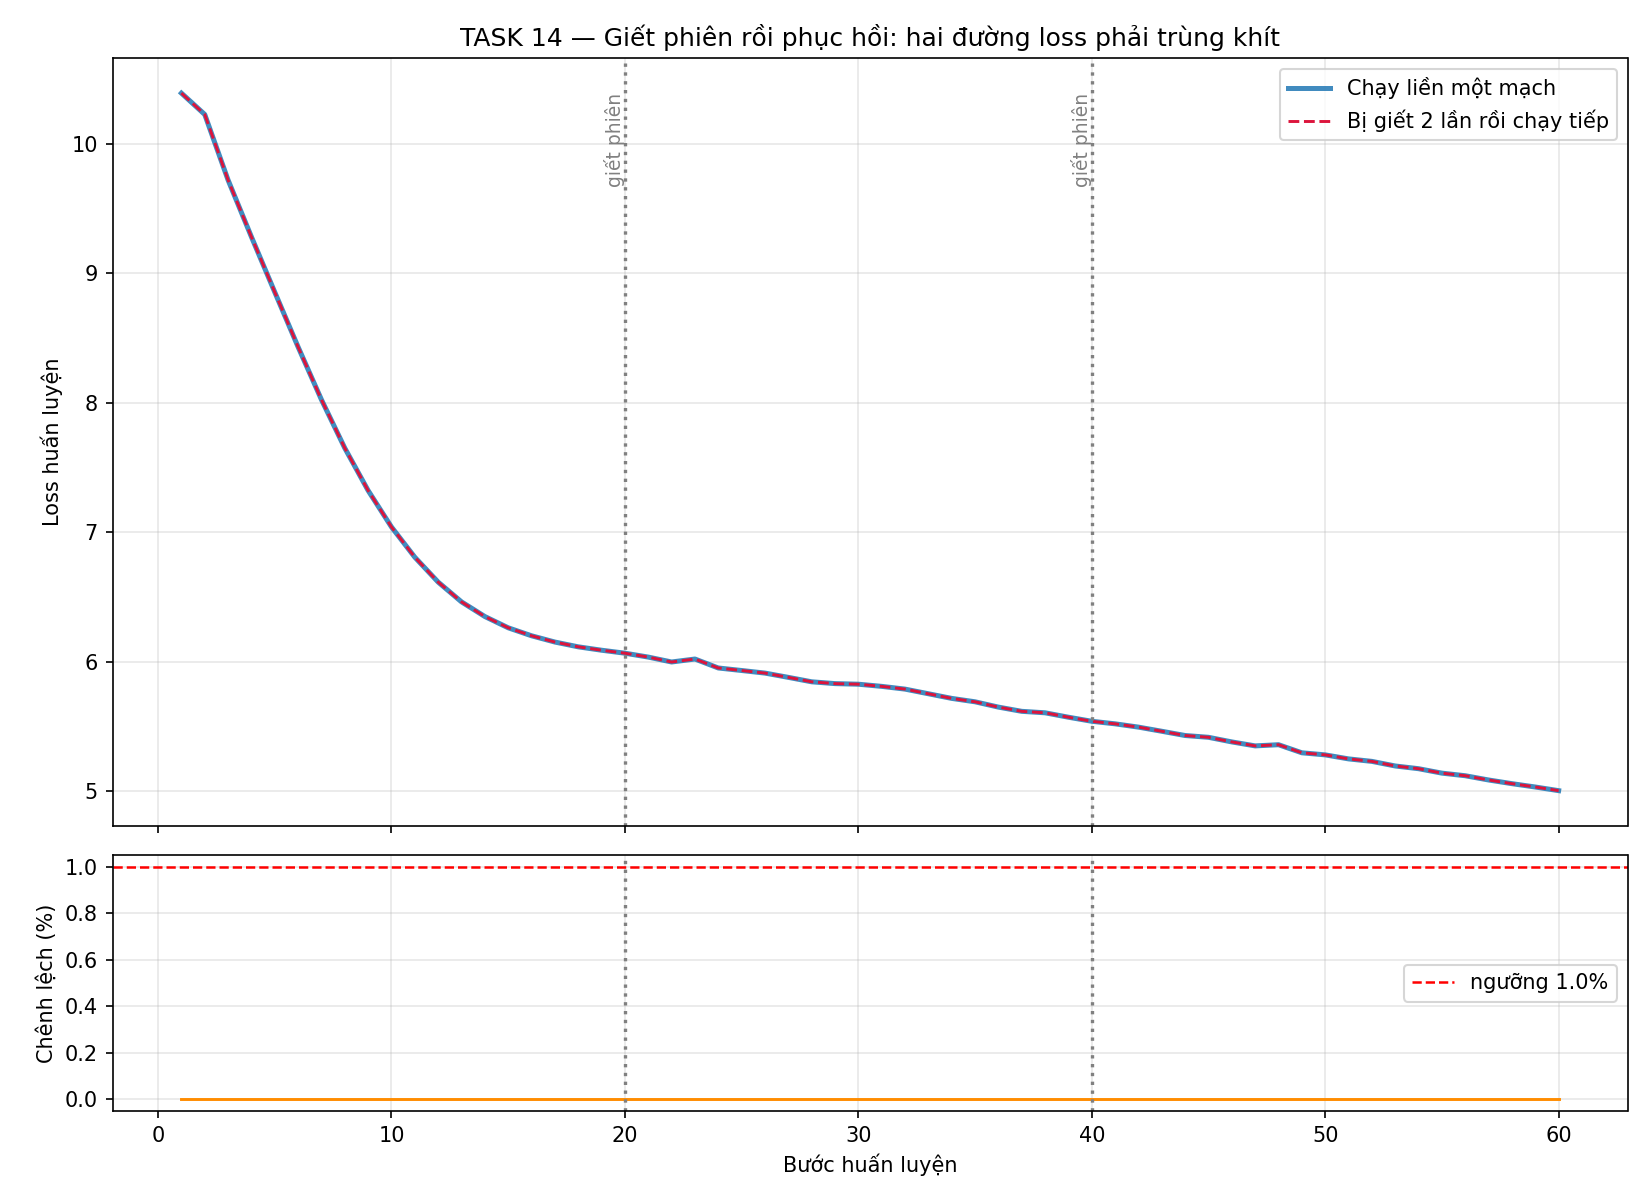
\includegraphics[width=0.88\textwidth]{thi_nghiem_phuc_hoi.png}
      \end{center}
      \vspace{-0.4em}
      {\scriptsize\textit{Hình 2: Lượt A chạy liền một mạch 60 bước; lượt B cùng seed
      nhưng bị giết ở bước 20 và 40, mỗi lần dựng lại từ số 0 rồi nạp checkpoint chạy
      tiếp — đúng như khi Kaggle ngắt phiên thật.}}
    \end{column}
    \begin{column}{0.41\textwidth}
      \begin{block}{Kết quả đo}
        \scriptsize\bangchat
        \begin{tabular}{@{}lr@{}}
          \toprule
          \textbf{Chỉ số} & \textbf{Giá trị} \\
          \midrule
          Số bước so sánh        & 60 \\
          Chênh lệch trung bình  & 0{,}0000\% \\
          \textbf{Chênh lệch lớn nhất} & \textbf{0{,}0000\%} \\
          Ngưỡng yêu cầu         & 1{,}0\% \\
          \midrule
          \textbf{Kết luận}      & \xong{} \\
          \bottomrule
        \end{tabular}
      \end{block}
      \begin{block}{Vì sao đây là hình quan trọng nhất}
        \footnotesize
        Hai đường \textbf{trùng khít} chứng minh checkpoint đã giữ đủ cả bảy món.
        Thiếu bất kỳ món nào thì hai đường tách dần ra mà \textbf{không có lỗi nào báo
        ra} — chỉ nhìn đồ thị mới phát hiện được.
      \end{block}
      \begin{beamercolorbox}[wd=\textwidth, rounded=true, sep=6pt]{block body alerted}
        {\color{MLIOTink}\footnotesize Thời gian lưu và đẩy checkpoint chiếm
        \textbf{0{,}01\%} tổng thời gian huấn luyện (yêu cầu $< 5\%$) — \xong{}.}
      \end{beamercolorbox}
    \end{column}
  \end{columns}
\end{frame}

% ------------------------------------------------------------
%  SLIDE 16 – Kết quả huấn luyện chính thức
% ------------------------------------------------------------
\begin{frame}[shrink=10]{Kết quả huấn luyện chính thức}
  \begin{columns}[T]
    \begin{column}{0.56\textwidth}
      \begin{center}
        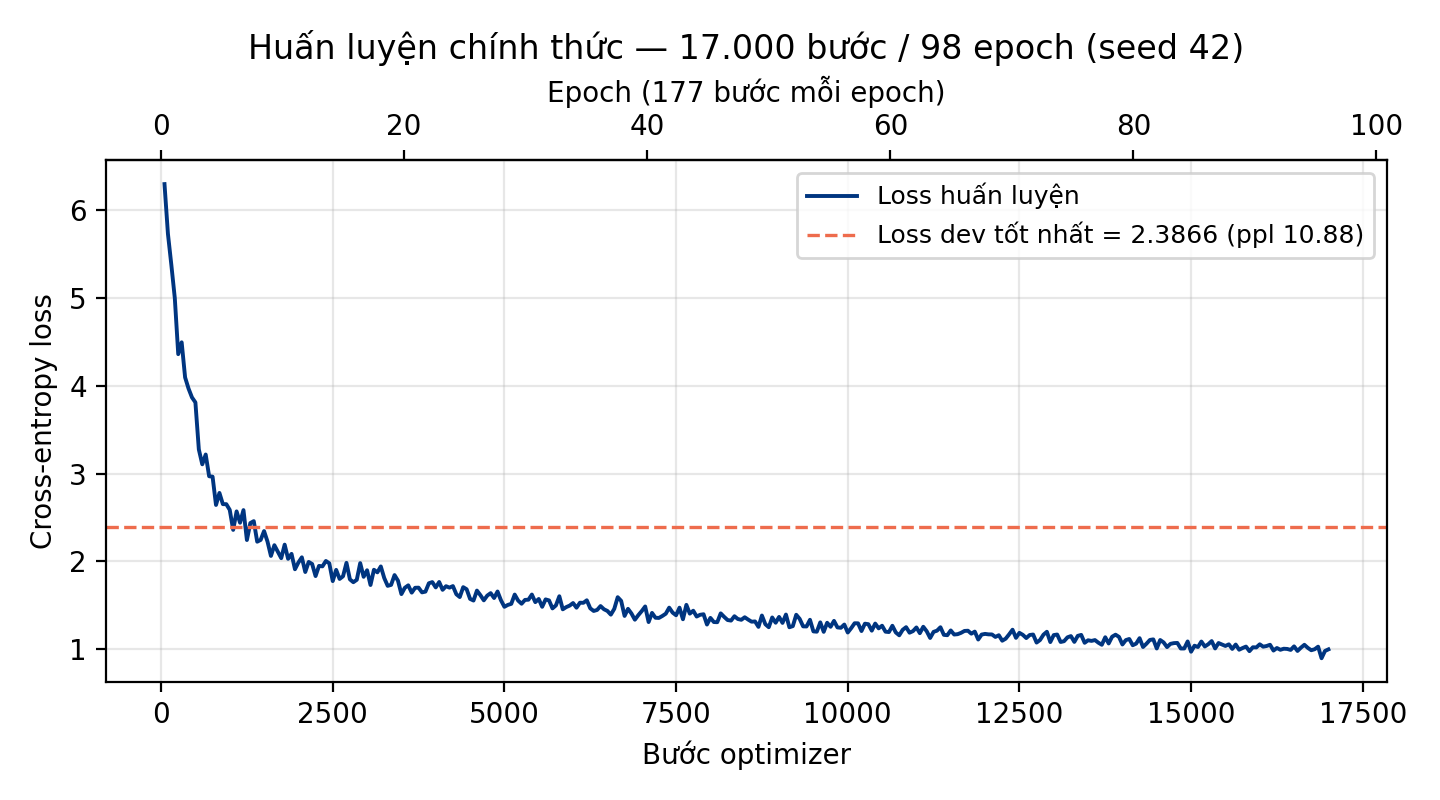
\includegraphics[width=\textwidth]{loss_huan_luyen.png}
      \end{center}
      \vspace{-0.3em}
      {\scriptsize\textit{Hình 3: Đường loss huấn luyện liền mạch qua nhiều phiên
      Kaggle — chính là bằng chứng cơ chế checkpoint hoạt động trong thực tế.}}
    \end{column}
    \begin{column}{0.4\textwidth}
      \begin{block}{Lượt chạy \texttt{iwslt\_base\_v1\_seed42}}
        \scriptsize\bangchat
        \begin{tabular}{@{}lr@{}}
          \toprule
          \textbf{Chỉ số} & \textbf{Giá trị} \\
          \midrule
          Tổng số bước               & 17.000 \\
          Số epoch                   & 98 \\
          Loss train cuối            & 0{,}9983 \\
          \textbf{Loss dev tốt nhất} & \textbf{2{,}3866} \\
          Perplexity dev             & 10{,}88 \\
          Dừng sớm                   & có \\
          Phiên cuối                 & 6.000 bước / 144{,}7 phút \\
          Tốc độ                     & ${\sim}13.800$ token/giây \\
          \bottomrule
        \end{tabular}
      \end{block}
      \begin{block}{Đọc con số này thế nào}
        \footnotesize
        \begin{itemize}
          \setlength{\itemsep}{0.15em}
          \item Loss train $0{,}998$ so với loss dev $2{,}387$ $\rightarrow$ mô hình đã
            \textbf{bắt đầu quá khớp}, đúng như dự đoán với 131k câu.
          \item \textbf{Dừng sớm} đã kích hoạt — cơ chế chống quá khớp làm đúng việc.
          \item Đáng chú ý: lượt ablation \textbf{3.000 bước} lại đạt loss dev
            \textbf{2{,}277} — \textit{tốt hơn} lượt 17.000 bước này. Chạy dài hơn
            5{,}7 lần mà tệ hơn, đúng vì quá khớp.
        \end{itemize}
      \end{block}
    \end{column}
  \end{columns}
\end{frame}

% ------------------------------------------------------------
%  SLIDE 17 – Chấm điểm và Ablation
% ------------------------------------------------------------
\begin{frame}[shrink=15]{Chấm điểm và Ablation}
  \begin{columns}[T]
    \begin{column}{0.48\textwidth}
      \begin{block}{Quy trình chấm điểm — hạ tầng đã sẵn sàng}
        \footnotesize
        \begin{itemize}
          \setlength{\itemsep}{0.15em}
          \item Chấm bằng \textbf{sacrebleu}: BLEU và chrF++, phải báo cáo
            \textbf{nguyên văn chuỗi chữ ký} thì mới so sánh được với người khác
          \item \textbf{Beam $=4$ hơn Greedy $+0{,}80$ BLEU} trên tst2013 (yêu cầu
            $\ge 0{,}50$) — đổi lại chậm hơn $1{,}8$ lần
          \item \textbf{KV cache}: ra \textbf{đúng cùng một chuỗi token} mà nhanh
            gấp \textbf{5{,}5 lần} ($20{,}3 \rightarrow 3{,}7$ giây) — cache chỉ
            được phép đổi tốc độ, có bài test đơn vị canh điều đó
          \item Hướng Anh $\rightarrow$ Việt, tập \textbf{tst2013}, \textbf{1.268} câu,
            chỉ dùng \textbf{một lần} ở bước cuối
        \end{itemize}
      \end{block}
      \begin{block}{Bảng điểm — Greedy vs Beam, cùng một checkpoint}
        \scriptsize\bangchat
        \begin{tabular}{@{}llccr@{}}
          \toprule
          \textbf{Tập} & \textbf{Sinh câu} & \textbf{BLEU} & \textbf{chrF++} &
          \textbf{Giây} \\
          \midrule
          tst2012 (dev)  & Greedy    & 25{,}41 & 44{,}77 & 8{,}9 \\
          tst2012 (dev)  & Beam $=4$ & 26{,}59 & 45{,}75 & 15{,}7 \\
          \midrule
          tst2013 (test) & Greedy    & 28{,}74 & 47{,}62 & 9{,}8 \\
          \textbf{tst2013 (test)} & \textbf{Beam $=4$} & \textbf{29{,}53} &
            \textbf{48{,}41} & 17{,}2 \\
          \bottomrule
        \end{tabular}
        \par\vspace{0.3em}
        {\tiny Chữ ký BLEU \texttt{nrefs:1\textbar case:mixed\textbar eff:no%
        \textbar tok:13a\textbar smooth:exp\textbar version:2.6.0}}
      \end{block}
    \end{column}
    \begin{column}{0.48\textwidth}
      \begin{block}{Ablation — mỗi thí nghiệm 2 seed, cùng 3.000 bước}
        \scriptsize\bangchat
        \begin{tabular}{@{}lccc@{}}
          \toprule
          \textbf{Cấu hình} & \textbf{BLEU tst2013} & \textbf{giây/bước} \\
          \midrule
          Đối chứng (RMSNorm) & $28{,}56 \pm 0{,}18$ & \textbf{1{,}511} \\
          \textbf{A1} (LayerNorm) & $28{,}60 \pm 0{,}27$ & 1{,}598 \\
          \midrule
          \textbf{A0} (vanilla 2017) & \multicolumn{2}{c}{\textit{đang chạy lại}} \\
          \bottomrule
        \end{tabular}
        \par\vspace{0.3em}
        Cùng ngân sách bước, chỉ đổi \textbf{đúng một yếu tố}, báo cáo cả độ lệch
        giữa hai seed.
      \end{block}
      \begin{beamercolorbox}[wd=\textwidth, rounded=true, sep=6pt]{block body alerted}
        {\color{MLIOTink}\footnotesize\textbf{A1 — trả lời câu mentor hỏi.}
        RMSNorm và LayerNorm chênh nhau \textbf{0{,}04 BLEU}, nhỏ hơn hẳn dao động
        giữa hai seed của chính từng nhóm ($0{,}18$ và $0{,}27$). Tức
        \textbf{chất lượng không phân biệt được}. Nhưng RMSNorm \textbf{nhanh hơn
        5{,}7\%}.
        \par\vspace{0.2em}
        Vậy lý do chọn RMSNorm là \textbf{tốc độ, không phải điểm số} — và đây là
        số đo của nhóm, không phải trích dẫn bài báo.}
      \end{beamercolorbox}
    \end{column}
  \end{columns}
\end{frame}

% ------------------------------------------------------------
%  SLIDE 18 – Kết luận
% ------------------------------------------------------------
\begin{frame}[shrink=15]{Kết luận}
  \begin{columns}[T]
    \begin{column}{0.52\textwidth}
      \begin{block}{Đã làm được}
        \footnotesize
        \begin{itemize}
          \setlength{\itemsep}{0.3em}
          \item \textbf{Kiến trúc tự viết hoàn chỉnh:} Transformer 47{,}96 triệu tham
            số với RoPE, RMSNorm, Pre-Norm và SwiGLU bằng PyTorch thuần —
            \textbf{12/12} bài kiểm tra \xong{}, lệch so với tham chiếu PyTorch
            $< 10^{-5}$.
          \item \textbf{Dữ liệu sạch, tái lập được:} 131.339 cặp câu, 24 cặp rò rỉ đã
            xóa khỏi train, tokenizer BPE 32k với tỉ lệ \tk{unk} bằng \textbf{0}.
          \item \textbf{Huấn luyện chịu lỗi thật sự:} 17.000 bước / 98 epoch qua nhiều
            phiên Kaggle, loss dev tốt nhất \textbf{2{,}3866} (ppl 10{,}88), phục hồi
            sau khi bị giết phiên lệch \textbf{0{,}0000\%}, chi phí đồng bộ
            \textbf{0{,}01\%}.
          \item \textbf{Chốt cấu hình bằng số đo:} 8 cấu hình đã khảo sát trên T4, chọn
            theo bảng chứ không theo bài báo.
          \item \textbf{Kết quả dịch:} Greedy \textbf{28{,}74} BLEU, Beam $=4$
            \textbf{29{,}53} BLEU và \textbf{48{,}41} chrF++ trên tst2013
            (sacrebleu) — \textbf{vượt mốc "rất tốt" $\ge 29$}, mà chỉ với
            \textbf{3.000 bước} và \textbf{chỉ dùng dữ liệu trong ràng buộc}.
        \end{itemize}
      \end{block}
    \end{column}
    \begin{column}{0.44\textwidth}
      \begin{block}{Còn dang dở}
        \footnotesize
        \begin{itemize}
          \setlength{\itemsep}{0.2em}
          \item A0 vanilla 2017 — đang chạy lại (lượt đầu đặt warmup 4.000 trong
            khi ngân sách chỉ 3.000 bước nên learning rate chưa từng lên tới đỉnh)
        \end{itemize}
      \end{block}
      \begin{beamercolorbox}[wd=\textwidth, rounded=true, sep=7pt]{block body alerted}
        \textbf{\textcolor{MLIOTblue}{Hướng phát triển:}}
        {\color{MLIOTink}\footnotesize
        \begin{itemize}
          \setlength{\itemsep}{0.1em}
          \item Chấm trên tst2015 để so trực tiếp với công bố IWSLT 2015
          \item Chống quá khớp mạnh hơn: label smoothing, dropout, back-translation
          \item Mở rộng sang PhoMT khi có ngân sách GPU lớn hơn
          \item Đóng gói Docker + Hugging Face Spaces và đo độ trễ đầu cuối
        \end{itemize}}
      \end{beamercolorbox}
    \end{column}
  \end{columns}
\end{frame}

% ------------------------------------------------------------
%  SLIDE 19 - Tai lieu tham khao (da gop 2 trang thanh 1)
% ------------------------------------------------------------
\begin{frame}[shrink=25]{Tài liệu tham khảo}
  \begin{columns}[T]
    \begin{column}{0.48\textwidth}
      \begin{thebibliography}{99}
        \setbeamertemplate{bibliography item}[text]
        \scriptsize

    \bibitem[1]{vaswani2017}
    Vaswani, A., Shazeer, N., Parmar, N., \textit{et al.} (2017).
    \textit{Attention Is All You Need.}
    NeurIPS 2017.
    arXiv: \href{https://arxiv.org/abs/1706.03762}{1706.03762}

    \bibitem[2]{su2024}
    Su, J., Ahmed, M., Lu, Y., Pan, S., Bo, W., Liu, Y. (2024).
    \textit{RoFormer: Enhanced Transformer with Rotary Position Embedding.}
    \textit{Neurocomputing}, 568, 127063.
    arXiv: \href{https://arxiv.org/abs/2104.09864}{2104.09864}

    \bibitem[3]{zhang2019}
    Zhang, B., Sennrich, R. (2019).
    \textit{Root Mean Square Layer Normalization.}
    NeurIPS 2019.
    arXiv: \href{https://arxiv.org/abs/1910.07467}{1910.07467}

    \bibitem[4]{shazeer2020}
    Shazeer, N. (2020).
    \textit{GLU Variants Improve Transformer.}
    arXiv: \href{https://arxiv.org/abs/2002.05202}{2002.05202}

    \bibitem[5]{xiong2020}
    Xiong, R., Yang, Y., He, D., \textit{et al.} (2020).
    \textit{On Layer Normalization in the Transformer Architecture.}
    ICML 2020.
    arXiv: \href{https://arxiv.org/abs/2002.04745}{2002.04745}

    \bibitem[6]{sennrich2016}
    Sennrich, R., Haddow, B., Birch, A. (2016).
    \textit{Neural Machine Translation of Rare Words with Subword Units.}
    ACL 2016, pp.\,1715--1725.
    arXiv: \href{https://arxiv.org/abs/1508.07909}{1508.07909}

      \end{thebibliography}
    \end{column}
    \begin{column}{0.48\textwidth}
      \begin{thebibliography}{99}
        \setbeamertemplate{bibliography item}[text]
        \scriptsize

    \bibitem[7]{micikevicius2018}
    Micikevicius, P., Narang, S., Alben, J., \textit{et al.} (2018).
    \textit{Mixed Precision Training.}
    ICLR 2018.
    arXiv: \href{https://arxiv.org/abs/1710.03740}{1710.03740}

    \bibitem[8]{loshchilov2019}
    Loshchilov, I., Hutter, F. (2019).
    \textit{Decoupled Weight Decay Regularization (AdamW).}
    ICLR 2019.
    arXiv: \href{https://arxiv.org/abs/1711.05101}{1711.05101}

    \bibitem[9]{post2018}
    Post, M. (2018).
    \textit{A Call for Clarity in Reporting BLEU Scores.}
    WMT 2018, pp.\,186--191.
    arXiv: \href{https://arxiv.org/abs/1804.08771}{1804.08771}

    \bibitem[10]{popovic2017}
    \tenlatin{Popovi\'{c}}, M. (2017).
    \textit{chrF++: words helping character n-grams.}
    WMT 2017, pp.\,612--618.

    \bibitem[11]{cettolo2015}
    Cettolo, M., Niehues, J., \tenlatin{St\"{u}ker}, S., Bentivogli, L., Cattoni, R.,
    Federico, M. (2015).
    \textit{The IWSLT 2015 Evaluation Campaign.}
    IWSLT 2015.

    \bibitem[12]{luong2015}
    Luong, M.-T., Manning, C.\,D. (2015).
    \textit{Stanford Neural Machine Translation Systems for Spoken Language Domains.}
    IWSLT 2015.

      \end{thebibliography}
    \end{column}
  \end{columns}

  \vspace{0.2em}
  {\scriptsize\textit{Mã nguồn và trọng số:}
  \href{https://github.com/giabaomaidev/bku-project}{github.com/giabaomaidev/bku-project}
  ·
  \href{https://huggingface.co/mgbao/envi-nmt-scratch-transformer}{huggingface.co/mgbao/envi-nmt-scratch-transformer}}
\end{frame}

% ------------------------------------------------------------
%  SLIDE 21 – Thank You / Acknowledgements
% ------------------------------------------------------------
\thankyouslide{%
  \textit{Nhóm xin cảm ơn thầy cô và mentor đã góp ý trực tiếp về warmup, label
  smoothing và việc chốt cấu hình bằng số liệu — những nhận xét đó đã định hình toàn
  bộ cách nhóm thiết kế phần ablation của đồ án.}
}

% ============================================================
\end{document}
% ============================================================
